%%%%%%%%%%%ESTUDIO DEL PROBLEMA%%%%%%%%%%%%%%%%
\chapter{Estudio del Problema}
	
	\section{Introducción}
	\par
	Como primera acción se analizó la factibilidad de implementación de un SoC con licencia OpenSource en FPGA, razón que condujo a la investigación del
	tópico en búsqueda de información necesaria que determine si existe tal posibilidad. Las características relevadas durante la investigación
	aportaron información respecto al hardware, las herramientas de desarrollo y el sistema operativo necesario para llevar a cabo la implementación. 
	\vspace{0.5cm}
	\par
	Para la selección del SoC se debió definir el microprocesador y los periféricos a utilizar, como así también las herramientas necesarias para la
	compilación y depuración de aplicaciones que corran sobre él. Esta situación derivó en una valoración de los diferentes entornos de desarrollo y
	sistemas operativos asociados que cumplan con el paradigma del software libre. Fue necesario además discernir entre las diversas alternativas de
	hardware que se tenían disponibles al momento del desarrollo de este trabajo compatibles con el SoC seleccionado. 
	\vspace{0.5cm}
	\par
	Fue necesario evaluar la posibilidad de implementar un Sistema Operativo que provea acceso mediante drivers a todos los periféricos conectados a
	la plataforma hardware elegida. La síntesis e implementación sobre FPGA requiere de aplicaciones específicas que debieron ponderarse para alcanzar el
	cumplimiento de los requerimientos.
	
	\newpage 
	
	\section{Requerimientos del Usuario}
	\par
	Se presenta en este apartado un listado de los requerimientos elecitados que tienen como objetivo comprender el dominio del problema y permiten
	trabajar en la realización de una solución eficiente.
	
		\subsection{En cuanto al Hardware}
		\begin{table}[h]
		\centering
		\begin{tabular}{ p{2.5cm} p{8cm} p{3cm} }
		\hline 
		\rowcolor[gray]{0.8} N\textordmasculine Req & Descripción & Tipo\\
		\hline
		RQX-HW 1 &  Se debe implementar un Microprocesador Softcore de núcleo simple & Cantidad y tipo de núcleos. \\
		\hline
		RQX-HW 2 &  El SoC seleccionado debe poseer la menor cantidad de restricciones respecto de su implementación en placas de desarrollo de diversos
		fabricantes. & Portabilidad a nivel Hardware\\
		\hline
		RQX-HW 3 & La placa de desarrollo elegida debe poseer al menos 32 MB de memoria RAM disponible que permita al ejecución del kernel de linux. &
		Memoria Disponible\\
		\hline
		RQX-HW 4 & La placa de desarrollo elegida debe poseer al menos 8 MB de memoria flash disponible que permita guardar la configuración de la FPGA y un
		bootloader & Memoria Disponible\\
		\hline
		\end{tabular}
		\caption{Listado de requerimientos de usuario - Hardware}
		\label{tab:requsr1}
		\end{table}
					
		\subsection{En cuanto a las Licencias}
		\begin{table}[h]
		\centering
		\begin{tabular}{ p{2.5cm} p{8cm} p{3cm} }
		\hline 
		\rowcolor[gray]{0.8} N\textordmasculine Req & Descripción  & Tipo\\
		\hline 
		RQX-LC 1 &  Todo el hardware implementado debe tener licencia LGPL o GPLv2 en su defecto & Licencias de hardware\\
		\hline 
		RQX-LC 2 &  Las herramientas de desarrollo utilizadas deben poseer licencias LGPL o GPLv2 en su defecto & Licencias de Software\\
		\hline
		RQX-LC 3 & El sistema operativo elegido debe poseer licencia LGPL o GPLv2 & Licencias de Software\\
		\hline
		\end{tabular}
		\caption{Listado de requerimientos de usuario - Licencias}
		\label{tab:requsr2}
		\end{table}
			
		\subsection{En cuanto a las Herramientas de Desarrollo}
		\begin{table}[h]
		\centering
		\begin{tabular}{ p{2.5cm} p{8cm} p{3cm} }
		\hline 
		\rowcolor[gray]{0.8} N\textordmasculine Req & Descripción  & Tipo\\
		\hline 
		RQX-HD 1 &  Las herramientas de desarrollo elegidas en base a la arquitectura a implementar deben tener la menor cantidad de restricciones respecto
		del sistema operativo donde serán ejecutadas & Portabilidad\\
		\hline 
		RQX-HD 2 &  Las herramientas de desarrollo deben brindar la capacidad de desarrollar y depurar programas para la arquitectura seleccionada &
		XXXXXXXXXXXX\\ % Revisar tipo de requerimiento
		\hline
		RQX-HD 3 &  Las herramientas de desarrollo de la placa seleccionada deben proveer soporte para el acceso a sus periféricos on board &
		XXXXXXXXXXXX\\ % Revisar tipo de requerimiento
		\hline 
		\end{tabular}
		\caption{Listado de requerimientos de usuario - Herramientas de Desarrollo}
		\label{tab:requsr3}
		\end{table}
		
		\subsection{En cuanto Sistema Operativo} 	 
		\begin{table}[h]
		\centering
		\begin{tabular}{ p{2.5cm} p{8cm} p{3cm} }
		\hline 
		\rowcolor[gray]{0.8} N\textordmasculine Req & Descripción  & Tipo\\
		\hline 
		RQX-SO 1 &  El sistema operativo elegido debe disponer de drivers y librerías que permitan el acceso a todos los dispositivos incluídos en el SoC &
		XXXXXXXXXXXXX\\ % Revisar tipo de requerimiento
		\hline 
		RQX-SO 2 &  El sistema operativo elegido debe tener la capacidad de ejecución multitarea e hilos & XXXXXXXXXXXX\\ % Revisar tipo de
		% requerimiento
		\hline
		RQX-SO 3 &  El sistema operativo elegido debe posibilitar la ejecución de aplicaciones de tiempo real & XXXXXXXXXXXX\\ % Revisar tipo de
		% requerimiento
		\hline 
		\end{tabular}
		\caption{Listado de requerimientos de usuario - Sistema Operativo}
		\label{tab:requsr4}
		\end{table}
	
	\section{Análisis de Riesgo}
		\subsection{Introducción}
        Para lograr producir aquello que se requiere, en el plazo solicitado y ajustados al presupuesto asignado, se necesita desarrollar
        un proceso que incluya desde la etapa más temprana la gestión de los riesgos asociados a los requerimientos, de forma que se contribuya al
        mejoramiento gradual del proceso de desarrollo y la gestión de un proyecto.
		\vspace{0.5cm}
		\par
        La gestión de riesgos procura formalizar conocimiento orientado a la minimización de riesgos en proyectos, mediante la
        generación de principios y buenas prácticas de aplicación realista \cite{etiqueta_riegos1}. Hasta el momento se ha propuesto
        y utilizado diferentes enfoques de gestión del riesgo desde que Boehm \cite{etiqueta_riegos2} atrajo a la comunidad de ingeniería del
        software hacia la gestión del riesgo. Sin embargo, es evidente que pocas organizaciones utilizan todavía de una forma explícita y sistemática
        métodos específicos para gestionar los riesgos en sus proyectos.
		\vspace{0.5cm}
		\par
        En \cite{etiqueta_riegos3} se presenta la definición de riesgo que plantea que el riesgo afecta a los futuros acontecimientos, implica
        cambios, e implica elección conjunto a la incertidumbre asociada a la misma. Es indiscutible que están presentes permanentemente las características de
        incertidumbre (acontecimiento que caracteriza al riesgo y que puede o no ocurrir) y de pérdida (si el riesgo se convierte en una realidad
        ocurrirán consecuencias no deseables o pérdidas).
		\vspace{0.5cm}
		\par
		Están definidas las categorías de riesgos: los riesgos del proyecto, que amenazan el plan; los riesgos técnicos, que amenazan la calidad y la
		planificación temporal; y los riesgos del negocio, que amenazan la viabilidad del proyecto o del producto. Otra categorización a considerar a
		partir del conocimiento que se tenga de ellos: los riesgos conocidos (los que se descubren en las evaluaciones); los riesgos predecibles (se
		extrapolan de la experiencia) y los riesgos impredecibles (pueden ocurrir, pero es muy difícil identificarlos de antemano).
		\vspace{0.5cm}
		\par
     	También son claras las estrategias frente al riesgo. Por un lado están las reactivas, cuyo método es evaluar las consecuencias del riesgo cuando
 		este ya se ha producido (ya no es un riesgo) y actuar en consecuencia. Este tipo de estrategias acarrea consecuencias negativas, al poner el
 		proyecto en peligro. Y por el otro las proactivas, que aplican el método de evaluación previa y sistemática de los riesgos y sus posibles
 		consecuencias, a la par que conforman planes de contingencias para de evitar y minimizar las consecuencias. Consecuentemente, este tipo de
 		estrategias permite lograr un menor tiempo de reacción ante la aparición de riesgos impredecibles.
		\vspace{0.5cm}
		\par
		De acuerdo con \cite{etiqueta_riegos3}, la administración o gestión de riesgos es un proceso iterativo que se aplica durante todo el proyecto y se
		desarrolla en cuatro etapas detalladas en la Figura ~\ref{fig:riesgos}. Se utilizó este modelo como guía para el análisis de los riegos del
		proyecto.
		
		\begin{figure}[!h]
 		\begin{center}
  		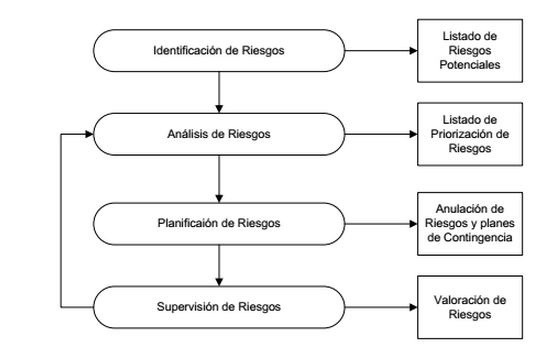
\includegraphics[width=0.8\textwidth,keepaspectratio=true]{./images/riesgos}
  		\caption{Procedimiento para la gestión de riesgos}
  		\label{fig:riesgos}
 		\end{center}
		\end{figure}
		
		\subsection{Identificación y análisis de riesgos}
		\par
		Se realizó un relevamiento inicial de riegos respecto de cada requerimiento de usuario planteado. Fue efectuado un análisis de severidad y
		probabilidad de ocurrencia para cada riesgo asociado. La severidad	del	impacto	de un riesgo concretado	se medió de la siguiente
		manera:
		
		\begin{itemize}
		  \item Catastrófico
		  \item Crítico	
		  \item Severo	
		  \item Menor	
		  \item Despreciable 
		\end{itemize}
	
		La probabilidad de ocurrencia se midió en base a la siguiente categorización:
	
		\begin{itemize}
		  \item Muy Probable
		  \item Probable	
		  \item Ocasional
		  \item Improbable 	
		  \item Remoto
		\end{itemize}
		
		En la Tabla ~\ref {tab:riegos} se listan los riesgos asociados, su severidad y probabilidad de ocurrencia para cada uno de los
		requerimientos de usuario.
		
		\begin{table}[!h]
		\centering
		\begin{tabular}{ p{2.5cm} p{9cm} p{2cm} p{2cm} }
		\hline 
		\rowcolor[gray]{0.8} N\textordmasculine Req & Riegos Asociados & Severidad  & Ocurrencia \\
		\hline
		RQX-HW 1& Código RTL con fallas reconocidas durante el proceso de síntesis & Crítica       & Probable \\
		\hline
				& Capacidad insuficiente para implementar la lógica del proyecto   & Catastrófico  & Ocasional\\	 
		\hline
		RQX-HW 2& Imposibilidad de acceso a alguno de los periféricos de la placa de desarrollo &  Crítica  & Probable\\
		\hline
		RQX-HW 3& Limitaciones de memoria RAM en las placas de desarrollo disponibles 	& Crítico  &  Improbable\\	 
		\hline
		RQX-HW 4& Limitaciones de memoria FLASH en las placas de desarrollo disponibles & Severo  &  Improbable\\ 
		\hline
		RQX-LC 1& Inexistencia de los Cores Open Source necesarios  	& Catastrófico  &  Ocasional\\
		\hline
				& Falta de documentación de apoyo para la implentación de los Cores  & Severo  &  Muy Probable\\ 
		\hline
		 		& Código RTL con fallas reconocidas durante el proceso de síntesis   & Critica & Probable\\ 
		\hline
		RQX-LC 2& Inexistencia de herramientas de desarrollo de hardware con licencias Open Source & Severo  &  Probable\\
		\hline
		RQX-LC 3& Inexistencia de herramientas de desarrollo de software con licencias Open Source & Severo  &  Improbable\\
		\hline
		RQX-LC 4& Inexistencia de un sistema operativo embebido con licencia Open Source  & Critico  &  Improbable\\
		\hline
		 		& Inexistencia de herramientas y librerias de sistema necesarias          & Critico  &  Probable\\
		\hline
		RQX-HD 1& Falta de herramientas de desarrollo portables a diversos sistemas operativos & Severo  &  Ocasional\\
		\hline		
		RQX-HD 2& Compilación cruzada incompatible con la arquitectura destino  & Critico &  Ocasional\\
		\hline
				& Falta de mecanismos de optimización de código del compilador  & Severo  &  Probable\\
		\hline
				& Imposibilidad de depuración de programas & Crítico  &  Probable\\
		\hline
		RQX-HD 3& Soporte de acceso a periféricos inexistente o con presencia de bugs & Critico &  Probable\\
		\hline
		RQX-SO 1& Drivers necesarios inexistentes o con fallos & Critico &  Probable\\
		\hline
				& Librerías necesarias inexistentes o con fallos & Severo &  Probable\\
		\hline
		RQX-SO 2& Incapacidad de ejección de hilos de los SO compatibles con el microprocesador elegido & Catastróficos & Improbable\\
		\hline
		RQX-SO 3& Limitaciones para la ejecución de SO de tiempo real & Critico & Probable\\
		\hline
		\end{tabular}
		\caption{Tabla de Riegos vs. Requerimientos}
		\label{tab:riegos}
		\end{table}
		
	\newpage	
			
	\section{Estudio de componentes}
		
			\subsection{Objetivo}
			Se estudiaron los componentes del proyecto y sus diversas alternativas de implementación por medio de un análisis comparativo que permitió evidenciar
			las características relevantes de cada uno de ellas. Inicialmente se realizó una comparativa de las prestaciones de los microprocesadores softcore
			más importantes para evaluar su capacidad de procesamiento. 
			
			\subsection{Selección del Microprocesador Soft-Core}
		
				\subsubsection{Comparación de Microprocesadores Soft-Core} 
	
				\subsubsection{Conclusiones de la elección del micro Soft-Core}
					 			
 			\subsection{Selección del SoC}
				\subsubsection{Comparación de proyectos SoC con procesador OpenRisc} 
				
				\paragraph{Proyecto MinSoC}
				La implementación llamada Minimal OpenRISC System on Chip utiliza IP cores estándar disponibles en OpenCores. Agrupa los cores necesarios para un
				SoC utilizando el procesador softcore OpenRISC OR1200. Este SoC puede ser sintetizado para cualquier FPGA y placa de desarrollo sin necesidad de
				realizar cambios en su descripción RTL. Para cumplir con esta premisa el proyecto se basa en una implementación básica de memoria y posee una
				unidad de debug llamada Advanced Debug System, que permite depurar el sistema y cargar los programas a ejecutar con la misma interfase utilizada
				para la configuración de la FPGA.
				
				El proyecto brinda soporte nativo a diversas placas y FPGAs mediante definiciones en el código RTL y archivos de constantes (constraint files)
				pero puede adaptarse a otras siguiendo una mínima serie de pasos. Se cuenta además con una serie testbenchs y firmwares que permiten realizar
				pruebas funcionales del sistema y son sirven de guía en los primeros desarrollos. Los testbenchs de MinSoC pueden ser ejecutados mediante la
				aplicación Icarus Verilog v.9.1. disponible en los repositorios estándar de la mayoría de las distribuciones Linux. 
				
				Existe una instancia de memoria on-chip de tamaño adaptable necesaria para soportar el firmware del CPU que conjuntamente con los cores que
				soportan los periféricos básicos son adaptados de acuerdo a las capacidades de la FPGA destino. 
				
				\paragraph{Proyecto ORPSoC}
				ORPSoC is the OpenRISC Reference Platform System-on-Chip. It is intended to be a development and verification environment for IP cores and SoC
				designs. It is a collaboratively developed project.
                As a development platform it should provide a modular, easy to use environment to perform RTL development with push-button simulation
                and synthesis flows. A basic software build environment is also present to support OpenRISC development in simulation and on target.
                The project should be easy enough for users, both new and experienced, to get started with OpenRISC designs and develop quickly and
                collaborate easily.
				
				
				
				\subsubsection{Conclusiones de la elección del micro Soft-Core}
 			
 			
 			\subsection{Selección de la Placa de Desarrollo}
 				\subsubsection{Análisis de las alternativas} 
				Los proyectos MinSoC y OrpSoc cuentan actualmente con soporte para diversas placas de desarrollo. 
				\paragraph{Xilinx}
				La empresa Xilinx provee kits de desarrollo de diversas características y prestaciones. A continuación se detallan algunas de las alternativas que
				son soportadas por los SoC elegidos.
				\subparagraph{S3ADSP1800A}
				El dispositivo XtremeDSP™ Starter Platform cuenta con una FPGA de la familia Spartan®-3A que permite la evaluación diseños para diferentes
				aplicaciones tales como Prototipado General, Sistemas Embebidos, Video Digital, DSP, Procesamiento de Imagenes, Comunicaciones digitales y
				Coprocesamiento. Esta plataforma provee acceso a las capacidades de la familia de FPGA Spartan®-3A y cuenta con periféricos,conectores e
				interfaces estándar de la industria. Fue diseñada para para ser utilizada con Xilinx System Generator para aplicaciones DSP y las herramientas de
				diseño ISE® o el entorno desarrollado en Linux llamado PetaLinux Software Development Kit (SDK) ambas herramientas provistas por el fabricante. 
				
				%Traducir esto ???
				Las características generales del kit son:
				
				\begin{tabular}{ p{4cm} p{10cm} }
				\rowcolor[gray]{0.8} Caracteristica & Descripción \\		
				\hline FPGA   & XC3SD1800A-4FGG676C Spartan-3A DSP FPGA\\
				\hline Clocks & 125 MHz LVTTL SMT oscillator\\
				\hline        & LVTTL oscillator socket\\
				\hline		  & 25.175 MHz LVTTL SMT oscillator (video clock)\\
				\hline		  & 25 MHz Ethernet clock (accessible to FPGA)\\
				\hline Memory & 128 MB (32M x 32) DDR2 SDRAM\\
				\hline		  & 16Mx8 parallel / BPI configuration flash\\
				\hline 		  & 64 Mb SPI configuration / storage flash (with 4 extra SPI selects)\\
				\hline Interfaces & 10/100/1000 PHY\\
				\hline			  & JTAG programming/configuration port\\
				\hline            & RS232 Port\\
				\hline			  & Low-cost VGA\\
				\hline			  & 4 SPI select lines\\
				\hline Buttons and Switches & 8 user LEDs\\
				\hline  		  & 8-position user DIP switch\\
				\hline            & 4 user push button switches\\
				\hline 			  & Reset push button switch\\
				\hline User I/O and Expansion & Digilent 6-pin header\\
				\hline			 			  & EXP expansion connector\\
				\hline 						  & 30-pin GPIO connector: can be used for System ACE™ Compact Flash daughter card (not included)\\
				\hline Configuration and Debug & JTAG\\
				\hline                         & System ACE module connector\\   
				\end{tabular}
				
				Las implementaciones MinSoC y ORPSoC proveen soporte nativo para los siguientes periféricos:
				
				\begin{itemize}
				  \item Ethernet
				  \item GPIO (Solo ORPSoC)
				  \item DDR2 SDRAM (128MB) (Solo ORPSoC)
				  \item SPI
				  \item UART				
				\end{itemize}
			
				\subparagraph{ML501}
				La ML501 es una plataforma de desarrollo de bajo costo y gran funcionalidad que provee un acceso práctico a los recursos disponibles en el
				dispositivo FPGA Virtex®-5 LX50. Posee interfases y conectores industriales estándar y presenta gran versatilidad para su utilización en
				múltiples aplicaciones como Video, Audio y puertos de comunicación.
				
				Las características generales del kit son:
			
			\begin{tabular}{ p{4cm} p{10cm} }
			\rowcolor[gray]{0.8} Caracteristica & Descripción \\		
			\hline FPGA & XC5VLX50FFG676\\
			\hline Memoria & DDR2 SODIMM (256 MB)\\
			\hline 		   & ZBT SRAM (1 MB)\\
			\hline 		   & Linear Flash (32 MB)\\
			\hline         & System ACE™ CF technology (Compact Flash)\\
			\hline         & Platform Flash\\
			\hline         & SPI Flash\\
			\hline Clocks  & External clocking (2 differential pairs)\\
			\hline Interfaces & USB (2) - host and peripheral\\
			\hline 			  & PS/2 (2) - keyboard, mouse\\
			\hline 			  & RJ-45 - 10/100 Networking\\
			\hline 			  & RS-232 (male) - serial port\\
			\hline 			  & Audio In (2) - line, microphone\\
			\hline 			  & Audio Out (2) - line, amp, SPDIF, piezo speaker\\
			\hline 			  & Video (DVI/VGA) Output\\
			\hline I/O y expansión & Single-ended and differential I/O expansion\\
			\hline GPIO		&  DIP switch (8)\\
			\hline 			&  LEDs (8)\\
			\hline 			&  push buttons (5)\\
			\hline Debug y programación & JTAG programming interface\\
			\hline Medioambiente & EU-RoHS compliant \\
			\end{tabular}
				
				Las implementación ORPSoC fue probada con éxito en esta plataforma y provee soporte para los siguientes periféricos:
				
				\begin{itemize}
				  \item Ethernet
				  \item GPIO
				  \item DDR2 SDRAM (256MB)
				  \item CFI flash (32MB)
				  \item SRAM
				  \item SPI
				  \item UART
				  \item AC97 
				  \item PS/2 				
				\end{itemize}
			
				
				\paragraph{Digilent}
				\subparagraph{Atlys}
				La placa de desarrollo Atlys es una plataforma que permite el desarrollo de circuitos digitales y esta soportada por una FPGA Xilinx Spartan 6
				LX45. Posee periféricos entre los que se destacan Gbit Ethernet, Video HDMI, Audio, puertos USB y Memoria Ram 128 MB DDR2 que permiten el
				desarrollo de Sistemas Digitales sobre procesadores embebidos como  MicroBlaze de Xilinx. Atlys es compatible con todas las herramientas CAD de
				Xilinx como ChipScope, EDK y WebPack (gratuito) lo que permite completar diseños sin mayor costo. Como alternativa puede utilizarse un entorno de
				desarrollo para Linux llamado PetaLinux Software Development Kit (SDK) provisto por el fabricante de la FPGA.
				
				Las características generales de la plataforma son:
				
				\begin{tabular}{ p{4cm} p{10cm} }
				\rowcolor[gray]{0.8} Caracteristica & Descripción \\		
				\hline FPGA   & Spartan-6 LX45, 324-pin BGA package \\
				\hline 		  &	6,822 slices each containing four 6-input LUTs and eight flip-flops\\
				\hline DSP	  & 58 DSP slices\\
				\hline Clocks & 2.1Mbits of fast block RAM\\
				\hline 		  & 4 clock tiles (8 DCMs \& 4 PLLs)\\
				\hline 		  & 6 phased-locked loops\\
				\hline 		  & 500MHz+ clock speeds\\
				\hline 		  & 100MHz CMOS oscillator\\
				\hline Memoria & 128Mbyte DDR2 16-bit wide data\\
				\hline         & 16Mbyte x4 SPI Flash for configuration \& data storage\\
				\hline GPIO & 8 LEDs \\
				\hline 		& 6 buttons\\
				\hline		& 8 slide switches\\
				\hline Interfaces & 10/100/1000 Ethernet PHY\\
				\hline 			  & On-board USB2 ports for programming \& data transfer\\
				\hline 			  & USB-UART and USB-HID port (for mouse/keyboard)\\
				\hline 			  & Two HDMI video input ports \& two HDMI output ports\\
				\hline			  & AC-97 Codec with line-in, line-out, mic, \& headphone\\
				\hline Energía & Real time power monitors on all power rails\\
				\hline 		   & 20W power supply and USB cable\\
				\hline I/O y Expansión & 48 I/O’s routed to expansion connectors\\
				\end{tabular}
				
				La implementación ORPSoC proveen soporte nativo para los siguientes periféricos:
				
				\begin{itemize}
				  \item AC97
				  \item Ethernet
				  \item GPIO
				  \item PS/2 
				  \item DDR2 SDRAM (128MB)
				  \item SPI
				  \item UART
				  \item VGA
				\end{itemize}				

				\paragraph{Terasic}
				\subparagraph{Terasic DE0 Nano}
				La plataforma DE0-Nano posee un tamaño compacto que se ajusta al diseño de circuitos para proyectos portables. Fue diseñada para ser
				utilizada con una implementación simple utilizando como destino una FPGA Cyclone IV de Altera con 22,320 LEs (Elementos Lógicos). Entre sus
				características princpiales se encuentran diversas interfases que incluyen dos puertos de expanxión GPIO, dispositivos de memoria on board SDRAM y
				EEPROM. Las mayores ventajas del DE0-Nano son su reducido tamaño y peso, así como la capacidad de ser reconfigurado sin la necesidad de
				utilización de hardware extra. Los requerimientos de energía para dispositivos portables son cruciales , la DE-0 Nano posee 3 esquemas posibles
				de conexión : un puerto USB mini-AB, conectores de 2 pines para alimentación externa de 5V, y 2 pines de 5V.

				Las características generales de la plataforma son:
				
				\begin{tabular}{ p{4cm} p{10cm} }
				\rowcolor[gray]{0.8} Caracteristica & Descripción \\		
				\hline FPGA   	& Cyclone® IV EP4CE22F17C6N FPGA\\
				\hline 			& 22,320 Logic elements (LEs)\\
				\hline 			& 594 Embedded memory (Kbits)\\
				\hline 			& 66 Embedded 18 x 18 multipliers\\
				\hline			& 4 General-purpose PLLs\\
				\hline 			& 153 Maximum FPGA I/O pins\\ 
				\hline Configuration Status and Set-Up Elements & 	On-board USB-Blaster circuit for programming\\
				\hline											&	FPGA Serial Configuration Device (EPCS)\\
				\hline Expansion Header & 	Two 40-pin Headers (GPIOs) provides 72 I/O pins\\
				\hline 					&	Two 5V power pins, two 3.3V power pins and four ground pins\\
				\hline 					&	One 26-pin header provides 16 digital I/O pins and 8 analog input pins to connect to analog sensors, etc\\ 
				\hline Memory Devices	&	32MB SDRAM\\
				\hline 					&	2Kb I2C EEPROM\\ 
				\hline General User Input/Output 	& 8 green LEDs\\
				\hline 								& 2 debounced push-buttons\\
				\hline 								& 4 dip switches\\ 
				\hline G-Sensor & ADI ADXL345, 3-axis accelerometer with high resolution (13-bit)\\ 
				\hline A/D Converter & NS ADC128S022, 8-Channel, 12-bit A/D Converter\\ 
				\hline					 & 50 ksps to 200 ksps \\
				\hline Clock System & On-board 50MHz clock oscillator\\
				\hline Power Supply & USB Type mini-AB port (5V)\\
				\hline 				& Two DC 5V pins of the GPIO headers (5V)\\
				\hline 				& 2-pin external power header (3.6-5.7V)\\
				\end{tabular}
				
				La implementación ORPSoC proveen soporte nativo para los siguientes periféricos:
				
				\begin{itemize}
				  	\item GPIO
					\item SDRAM (32MB)
					\item UART
					\item SPI FLASH (8MB)
					\item I2C
				\end{itemize}				
				
 				\subsubsection{Conclusiones de la elección de la Placa de Desarrollo}
 				Se seleccionó entre los items analizados y teniendo en cuenta la disponibilidad de recursos al momento de realizar este trabajo utilizar las
 				placas S3ADSP1800A de Xilinx para soportar los SoC a implementar.
 			
 			\subsection{Selección de las herramientas de desarrollo} 	 
 		
 		
 			\subsection{Selección del Sistema Operativo}
 			